\documentclass[12pt,a4paper]{article}

% Pakiety językowe i kodowanie
\usepackage[utf8]{inputenc}
\usepackage[T1]{fontenc}
\usepackage[polish]{babel}

% Pakiety matematyczne i graficzne
\usepackage{amsmath}
\usepackage{amsfonts}
\usepackage{amssymb}
\usepackage{graphicx}
\usepackage{float}
\usepackage{geometry}

% Optymalne marginesy
\geometry{margin=2.0cm}

\title{Sprawozdanie: Obliczenia i własności w grupach permutacji}
\author{Franciszek Szarek, 183962}
\date{\today}

\begin{document}

\maketitle

\tableofcontents
\clearpage

\section{Wprowadzenie}
Niniejsze sprawozdanie dokumentuje serię obliczeń na permutacjach w grupie symetrycznej $S_n$. Wykonywane operacje obejmują składanie permutacji, potęgowanie, odwracanie, rozwiązywanie równań, badanie struktury cyklowej (inwolucje) oraz wyznaczanie inwersji. Wszystkie analityczne obliczenia przeprowadzone ręcznie zostały zweryfikowane za pomocą systemu algebry komputerowej Maxima.

\section{Zadanie 2: Operacje algebraiczne na permutacjach}

Celem zadania było obliczenie skomplikowanego wyrażenia algebraicznego składającego się z wielu permutacji, w tym potęgowanych oraz poddawanych operacji odwrotności. Ze względu na obszerność, obliczenia podzielono na etapy.

\begin{figure}[H]
    \centering
    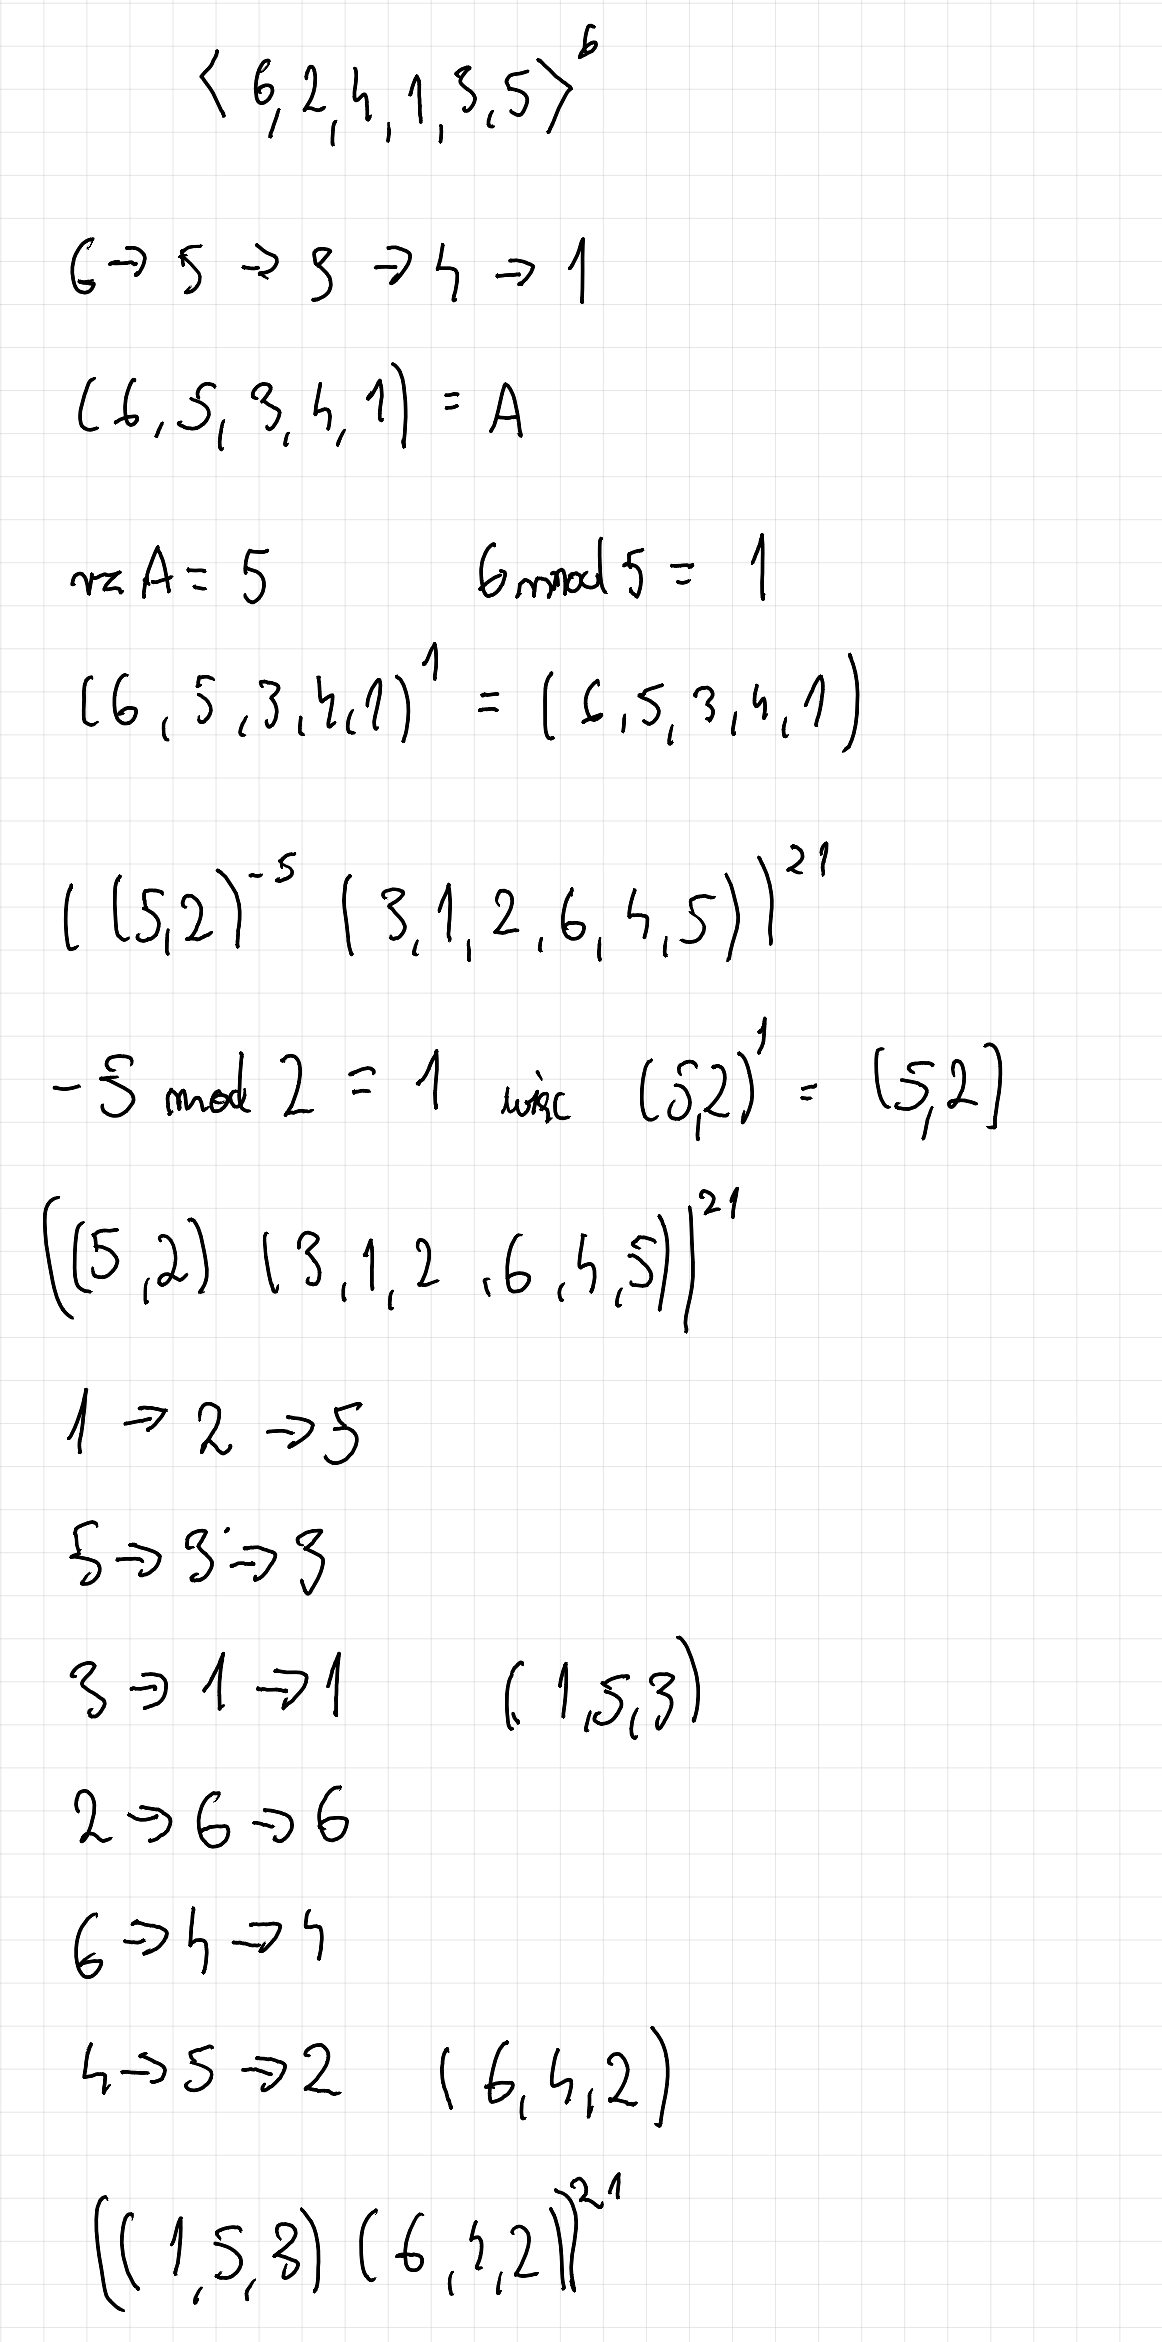
\includegraphics[width=0.45\textwidth]{zad 2_1.png}
    \caption{Zadanie 2 -- Etap I: Redukcja wykładników i potęgowanie cykli.}
    \label{fig:zad2_1}
\end{figure}

\textbf{Opis do Rysunku \ref{fig:zad2_1}:}
W pierwszej fazie obliczeń zajęto się początkowymi elementami wyrażenia. Zastosowano kluczową własność rzędu permutacji do zredukowania wysokich wykładników potęg (np. $6 \pmod 5 = 1$). Obliczono również odwrotność permutacji podniesionej do potęgi ujemnej.

\begin{figure}[H]
    \centering
    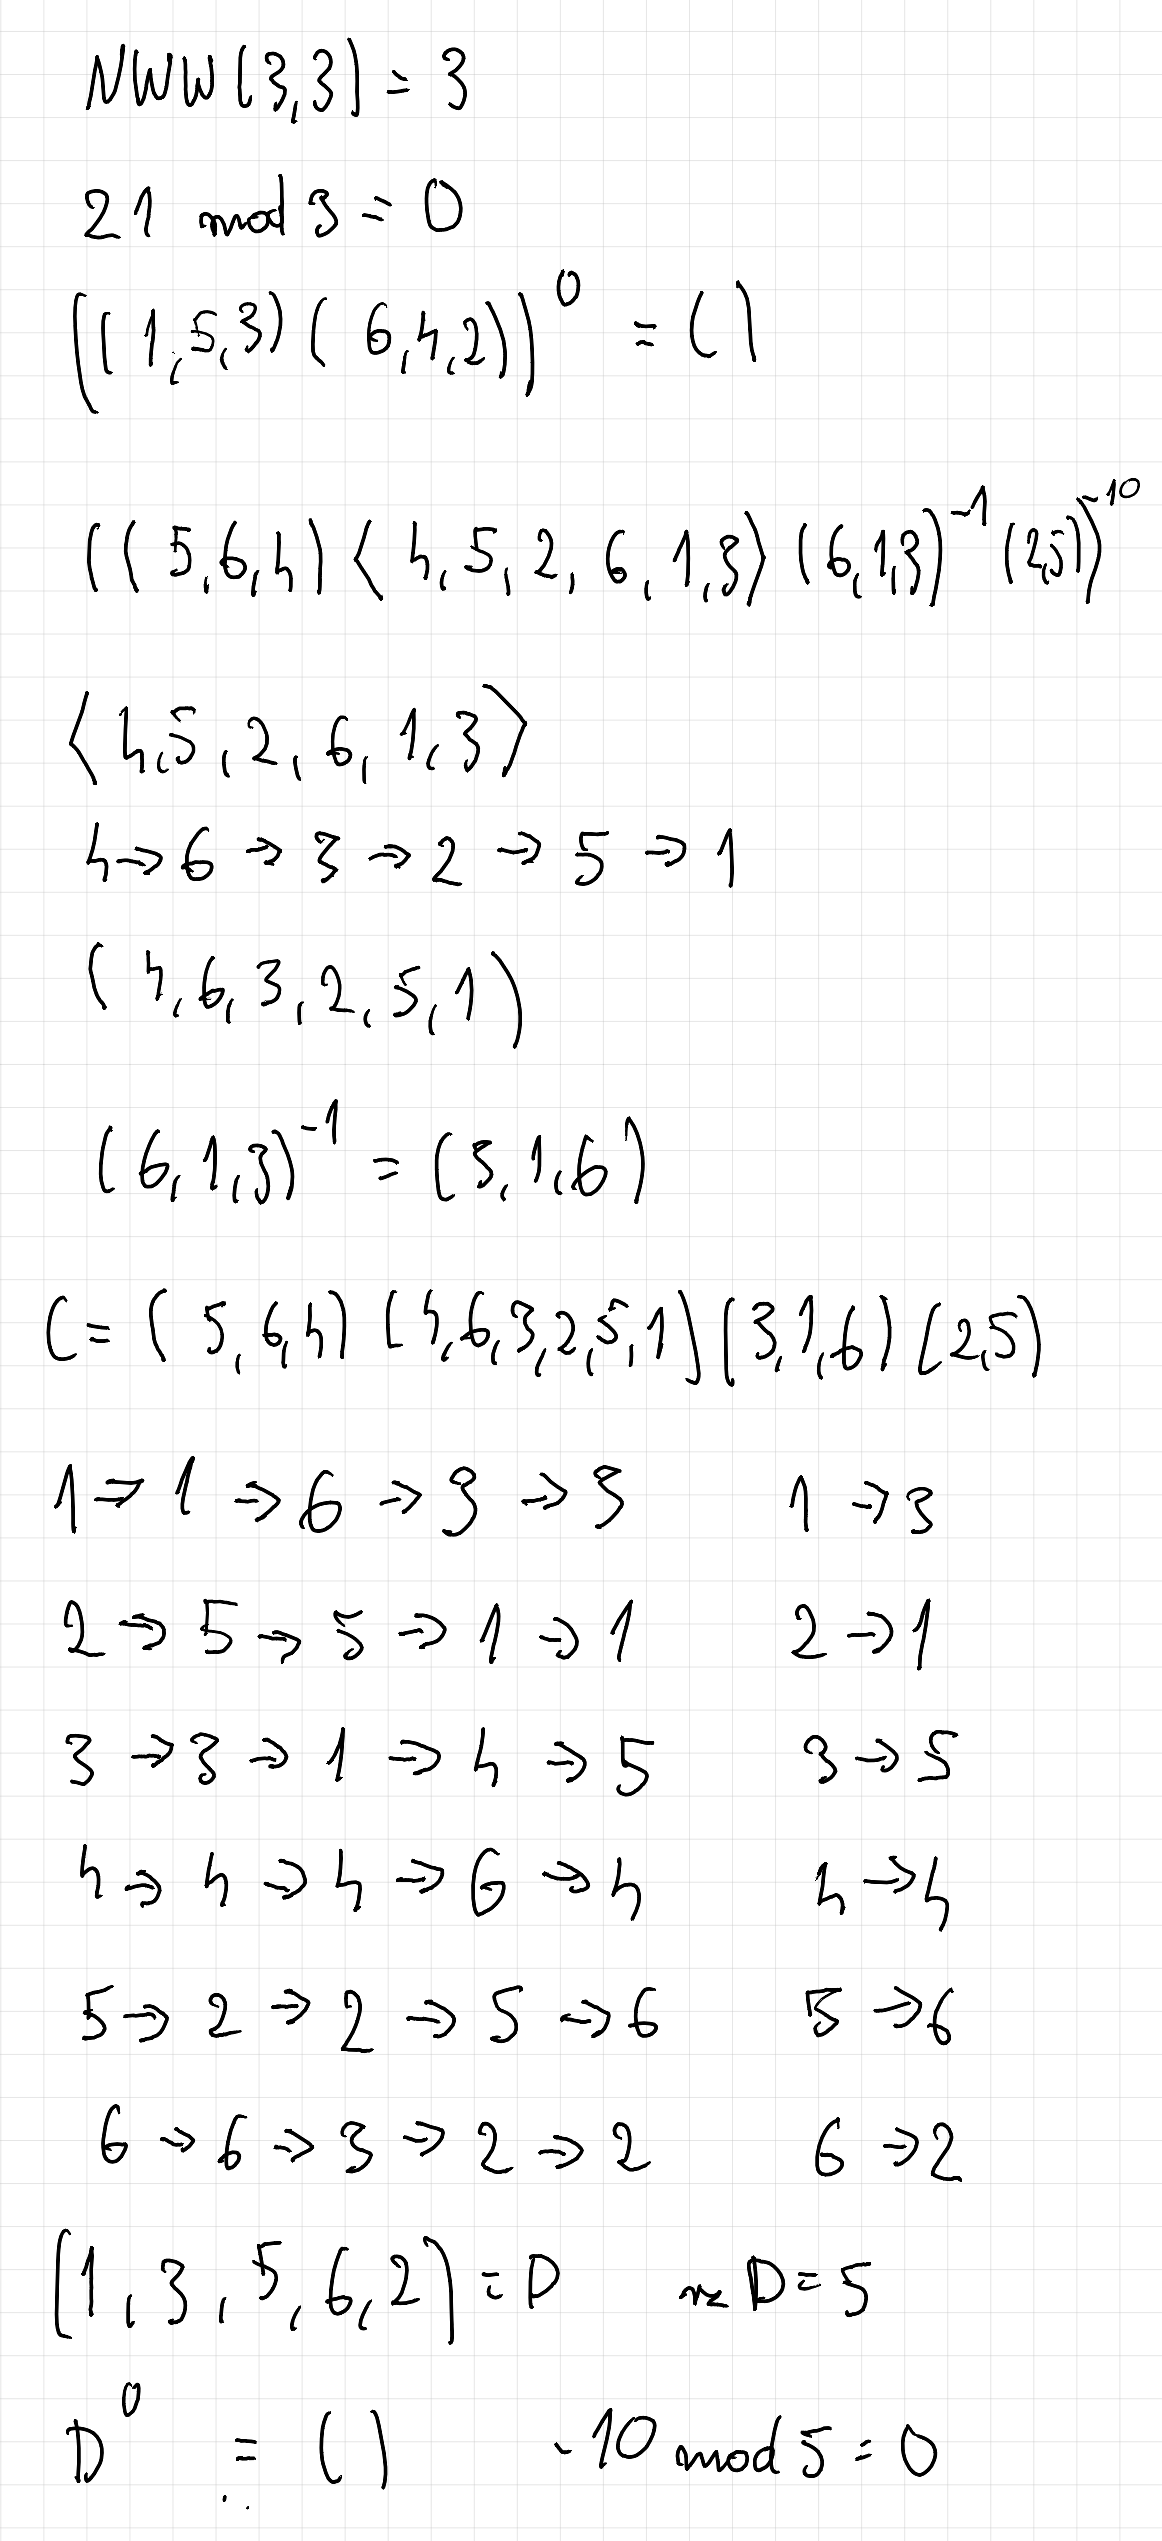
\includegraphics[width=0.45\textwidth]{zad 2_2.png}
    \caption{Zadanie 2 -- Etap II: Upraszczanie dalszych potęg i cykli.}
    \label{fig:zad2_2}
\end{figure}

\textbf{Opis do Rysunku \ref{fig:zad2_2}:}
W drugim kroku kontynuowano redukcję. Zauważono, że potęga z rzędu $21$ dla permutacji o rzędzie $3$ (NWW długości cykli) daje resztę $0$, co sprowadza ten fragment wyrażenia do permutacji identycznościowej $()$. Uproszczono kolejne nawiasy, przygotowując składowe do ostatecznego wymnożenia.

\begin{figure}[H]
    \centering
    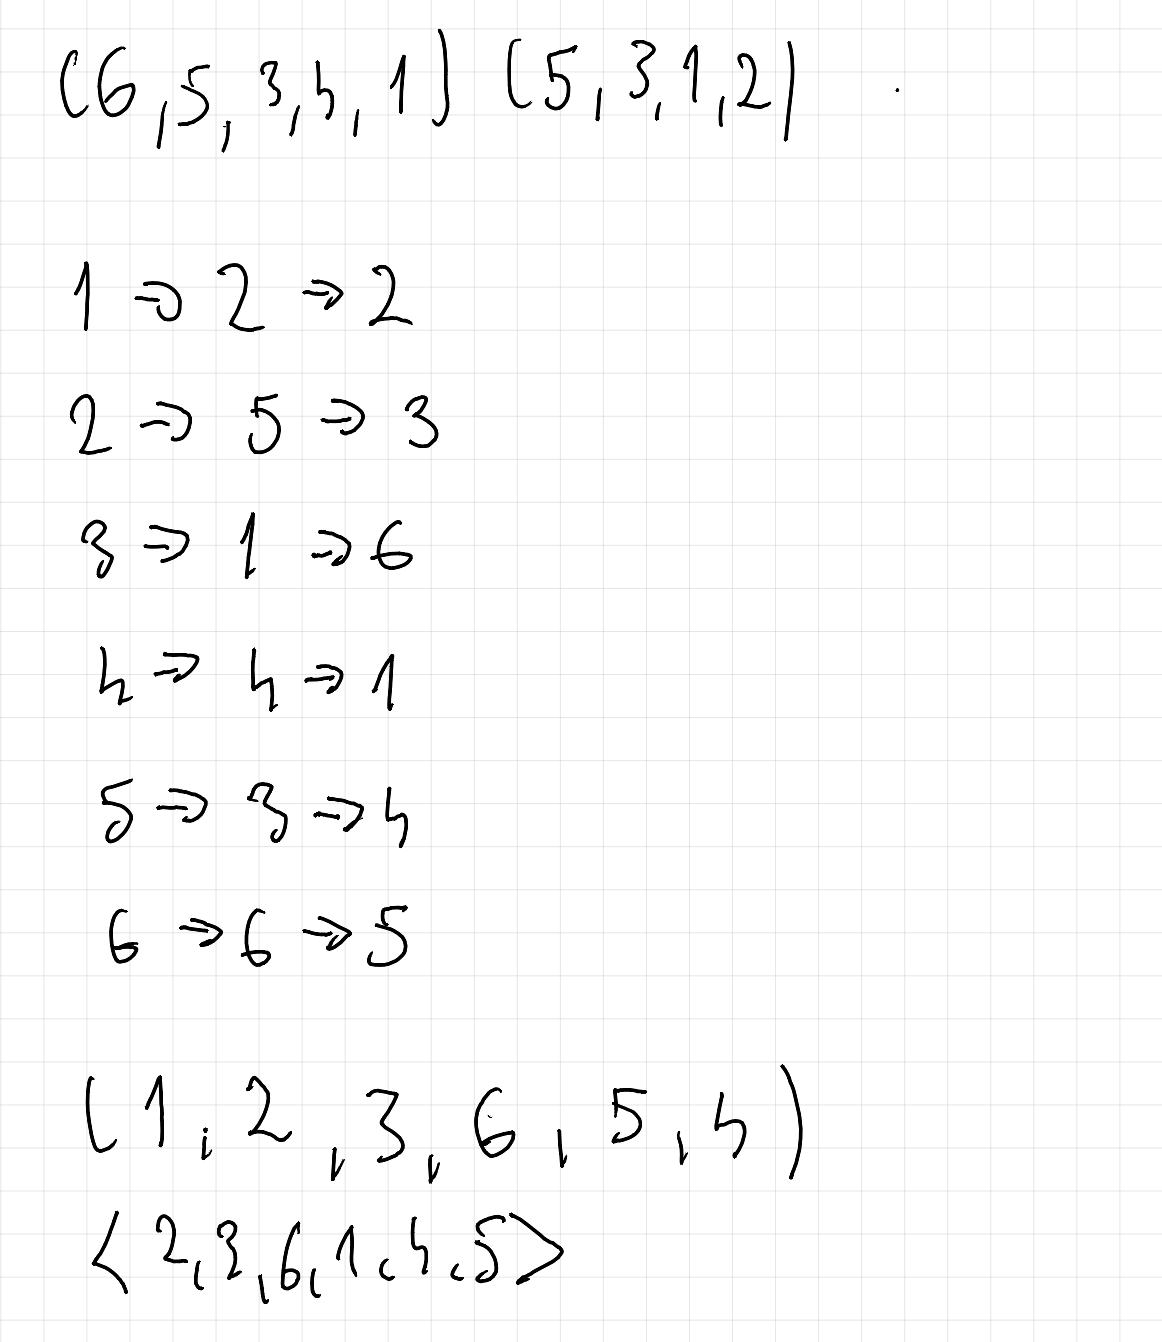
\includegraphics[width=0.45\textwidth]{zad 2_3.png}
    \caption{Zadanie 2 -- Etap III: Końcowe składanie permutacji i wynik.}
    \label{fig:zad2_3}
\end{figure}

\textbf{Opis do Rysunku \ref{fig:zad2_3}:}
Ostatni etap ręcznych wyliczeń to złożenie (wymnożenie) przygotowanych wcześniej permutacji od strony prawej do lewej. Po prześledzeniu przejść dla każdego elementu od $1$ do $6$, otrzymano końcowy wynik w notacji jednowierszowej: $\langle 2, 3, 6, 1, 4, 5 \rangle$.

\begin{figure}[H]
    \centering
    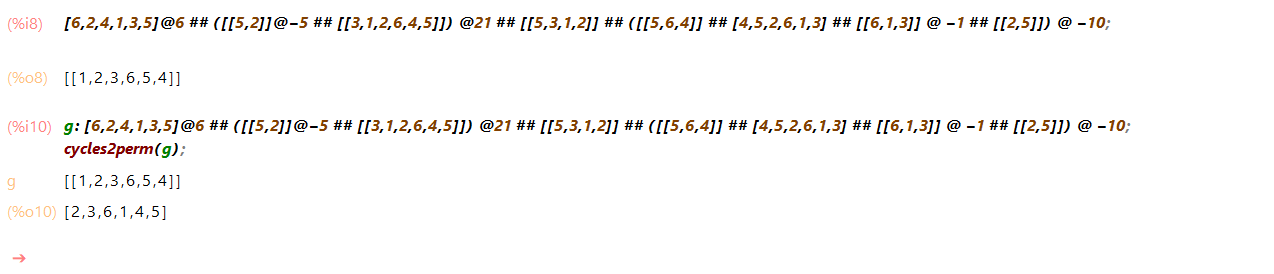
\includegraphics[width=0.9\textwidth]{zad 2 maxima.png}
    \caption{Weryfikacja Zadania 2 w systemie Maxima.}
    \label{fig:zad2_maxima}
\end{figure}

\textbf{Opis do Rysunku \ref{fig:zad2_maxima}:}
Równanie zostało wyliczone z użyciem programu Maxima. Otrzymany wynik w notacji listowej \texttt{[2,3,6,1,4,5]} w pełni pokrywa się z wartością wyznaczoną analitycznie.

\clearpage

\section{Zadanie 3a: Rozwiązywanie równań w grupie permutacji}

W tym zadaniu należało rozwiązać algebraiczne równanie postaci $L = P$ z niewiadomą permutacją $p$.

\begin{figure}[H]
    \centering
    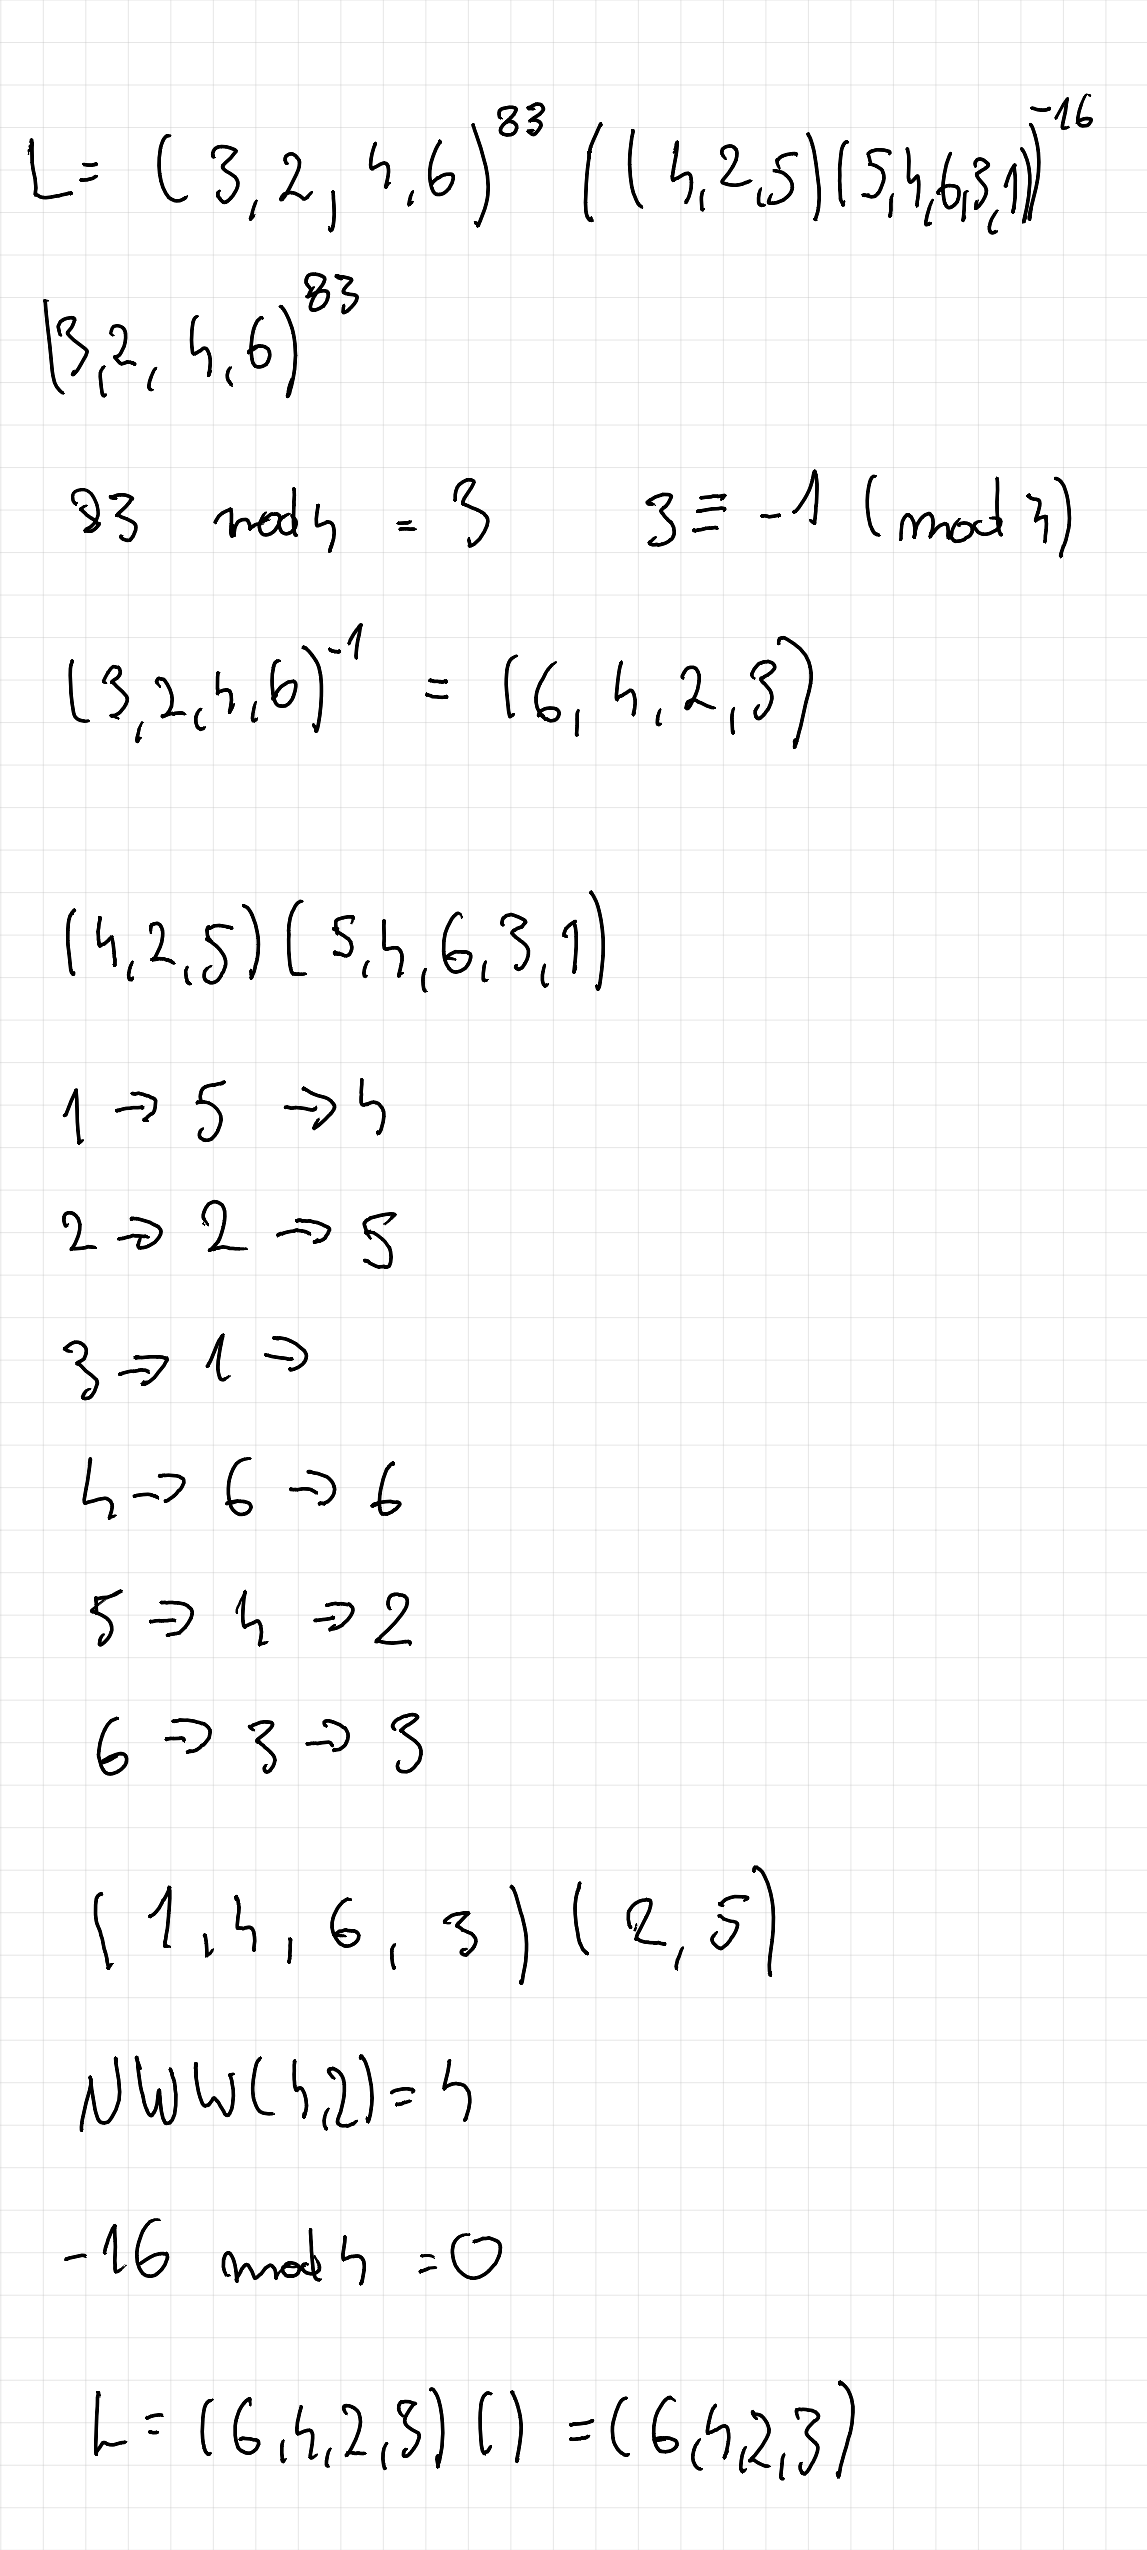
\includegraphics[width=0.4\textwidth]{zad 3a_1.png}
    \caption{Zadanie 3a -- Etap I: Obliczanie lewej strony równania (L).}
    \label{fig:zad3a_1}
\end{figure}

\textbf{Opis do Rysunku \ref{fig:zad3a_1}:}
Rozwiązywanie rozpoczęto od uproszczenia lewej strony równania ($L$). Podobnie jak w poprzednim zadaniu, zredukowano potęgi z wykorzystaniem operacji modulo (np. $83 \pmod 4 = 3 \equiv -1 \pmod 4$). Lewą stronę sprowadzono do pojedynczej permutacji $(6, 4, 2, 3)$.

\begin{figure}[H]
    \centering
    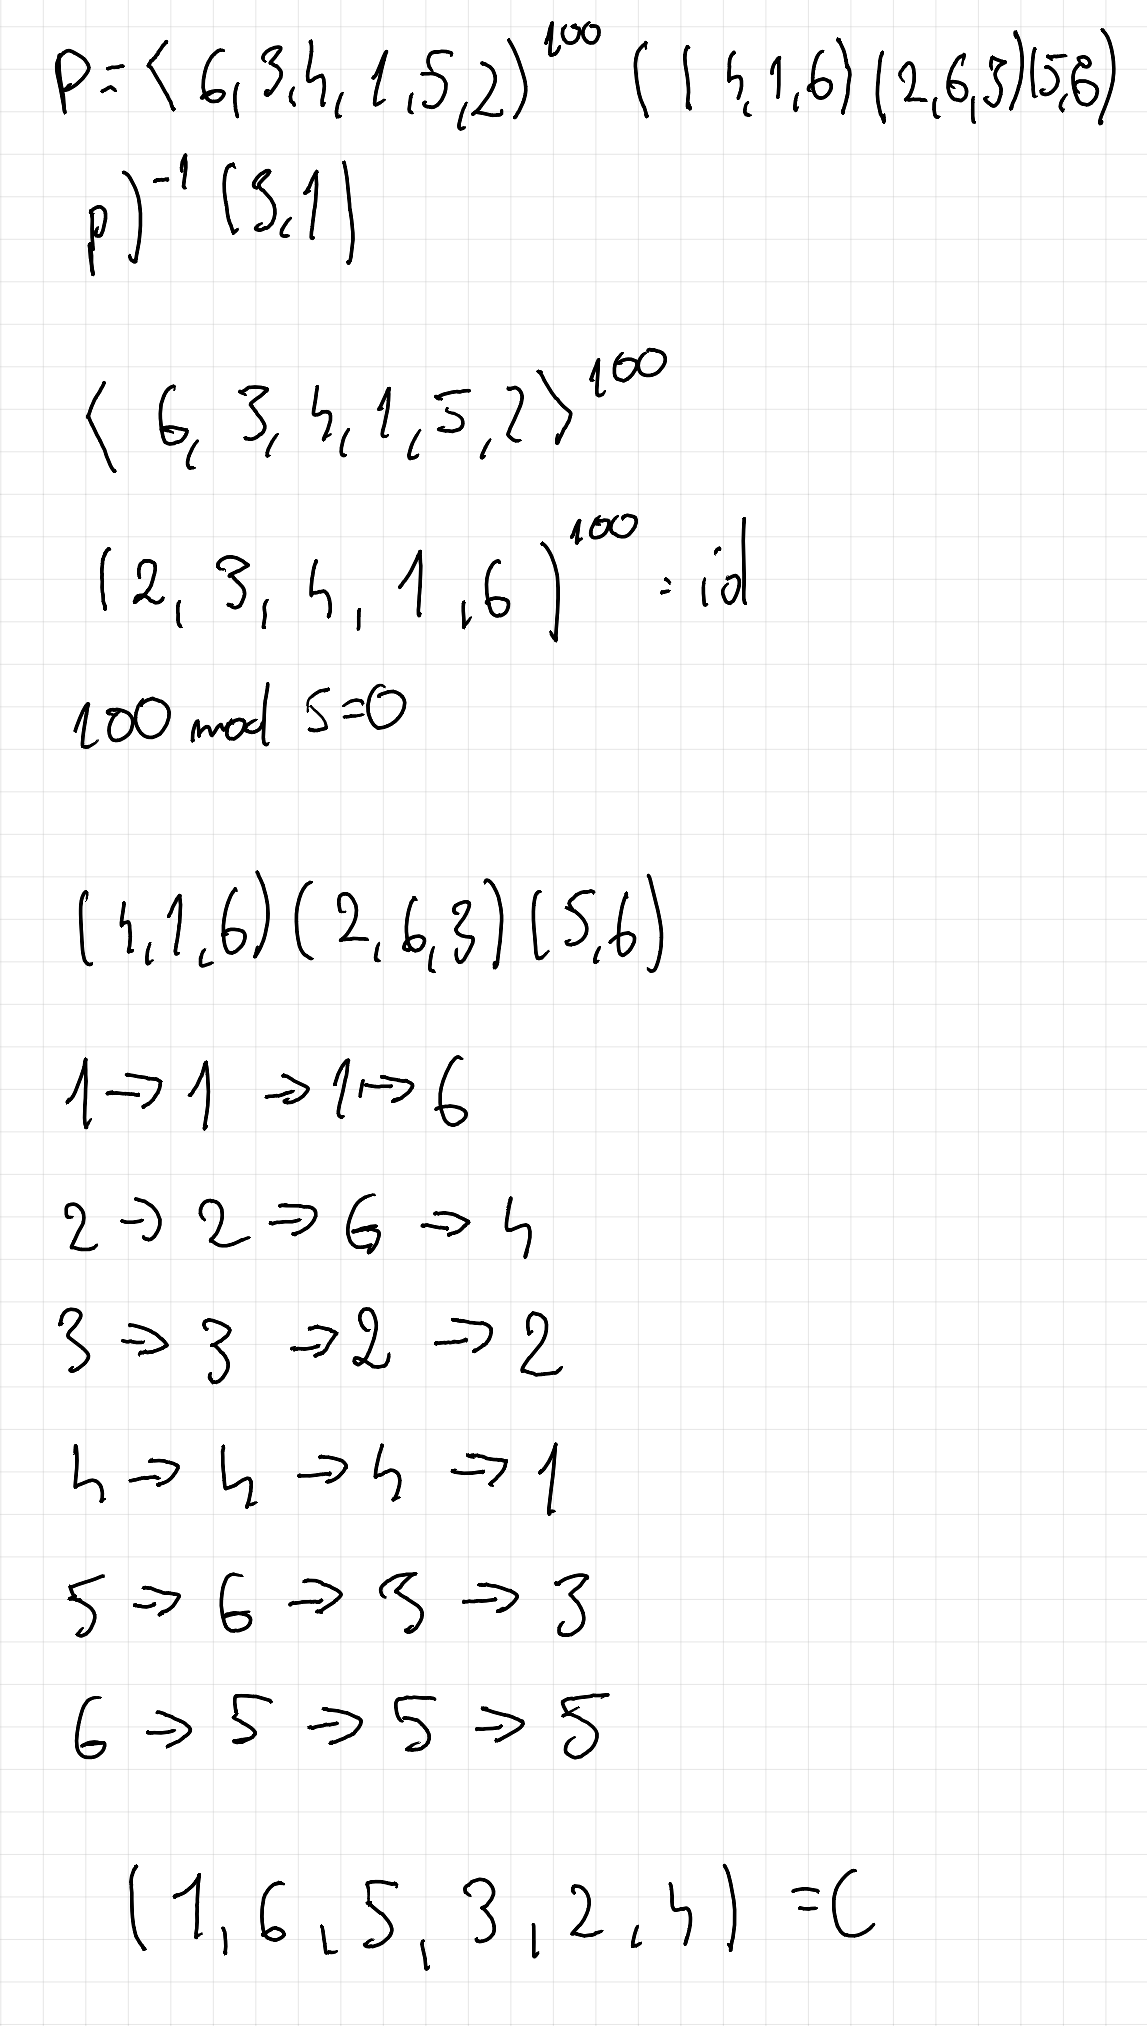
\includegraphics[width=0.45\textwidth]{zad 3a_2.png}
    \caption{Zadanie 3a -- Etap II: Upraszczanie prawej strony równania (P).}
    \label{fig:zad3a_2}
\end{figure}

\textbf{Opis do Rysunku \ref{fig:zad3a_2}:}
Prawa strona równania zawierała poszukiwaną niewiadomą $p$. Skrócono element podniesiony do setnej potęgi (wynik to identyczność, gdyż $100 \pmod 5 = 0$). Złożono pozostałe, znane cykle po obu stronach niewiadomej, co pozwoliło zapisać równanie w czytelniejszej postaci przed jego ostatecznym przekształceniem.

\begin{figure}[H]
    \centering
    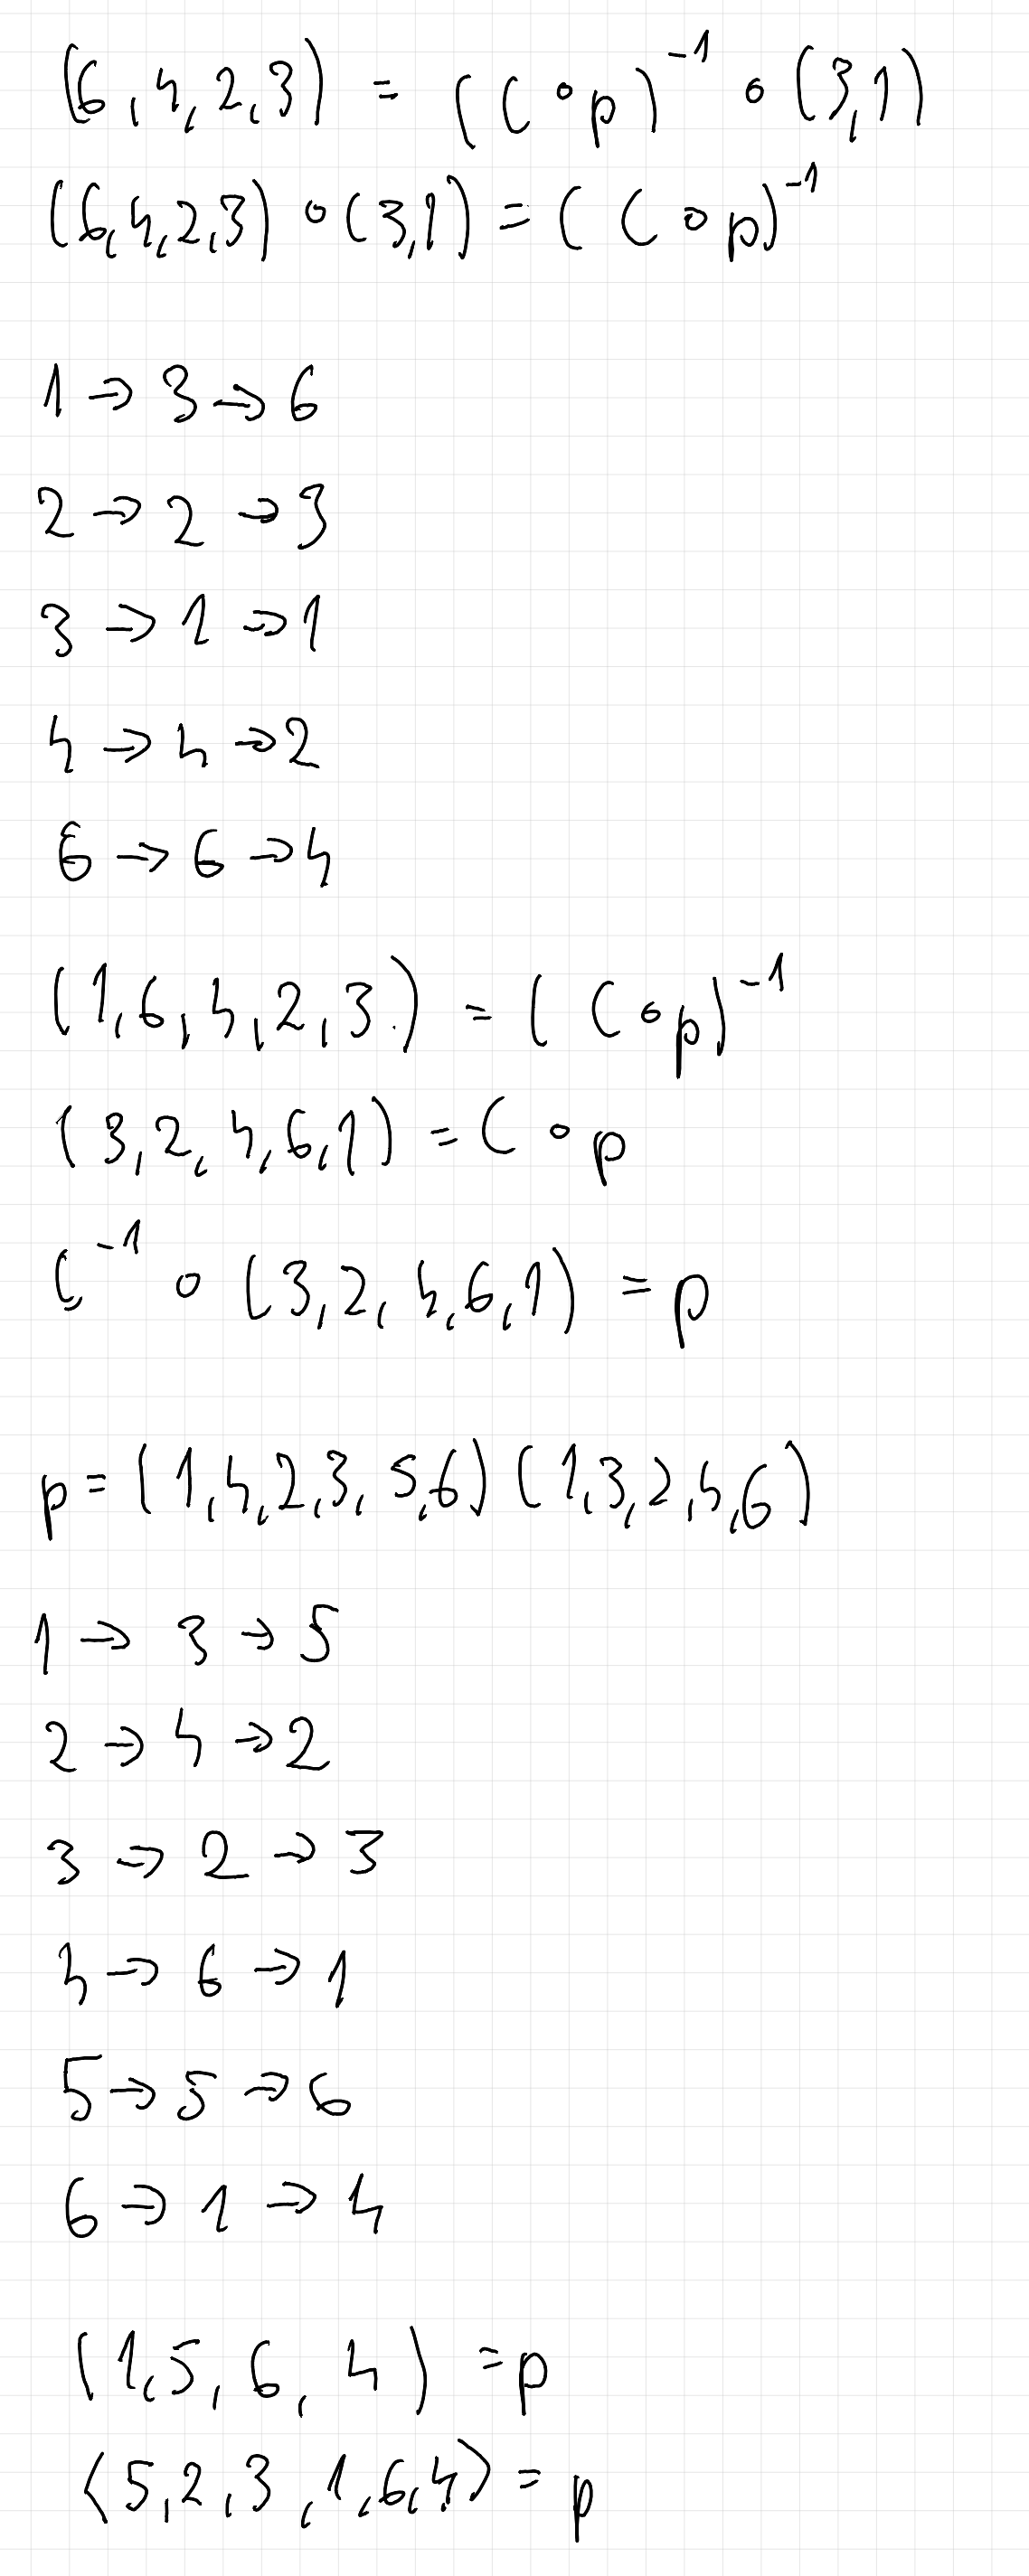
\includegraphics[width=0.45\textwidth]{zad 3a_3.png}
    \caption{Zadanie 3a -- Etap III: Wyizolowanie i wyliczenie niewiadomej $p$.}
    \label{fig:zad3a_3}
\end{figure}

\textbf{Opis do Rysunku \ref{fig:zad3a_3}:}
Aby wyznaczyć $p$, równanie pomnożono obustronnie (z odpowiednich stron) przez permutacje odwrotne do tych, które otaczały niewiadomą. Po wykonaniu ostatecznego składania cykli, uzyskano wynik $p = \langle 5, 2, 3, 1, 6, 4 \rangle$.

\begin{figure}[H]
    \centering
    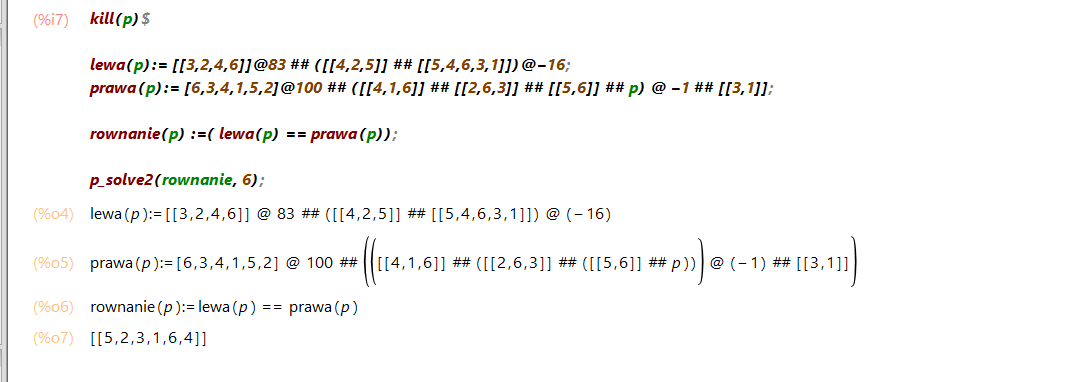
\includegraphics[width=0.9\textwidth]{zad 3a maxima.png}
    \caption{Rozwiązanie równania za pomocą Maximy.}
    \label{fig:zad3a_maxima}
\end{figure}

\textbf{Opis do Rysunku \ref{fig:zad3a_maxima}:}
Zadeklarowano zmienne reprezentujące lewą i prawą stronę równania, a następnie użyto wbudowanego solwera. Wynik \texttt{[5,2,3,1,6,4]} potwierdził wcześniejsze obliczenia ręczne.

\clearpage

\section{Zadanie 3b: Zliczanie inwolucji w grupach symetrycznych}

Inwolucje to permutacje, które są odwrotne same do siebie. Oznacza to, że ich rozkład na cykle rozłączne może zawierać wyłącznie cykle długości 1 lub 2.

\begin{figure}[H]
    \centering
    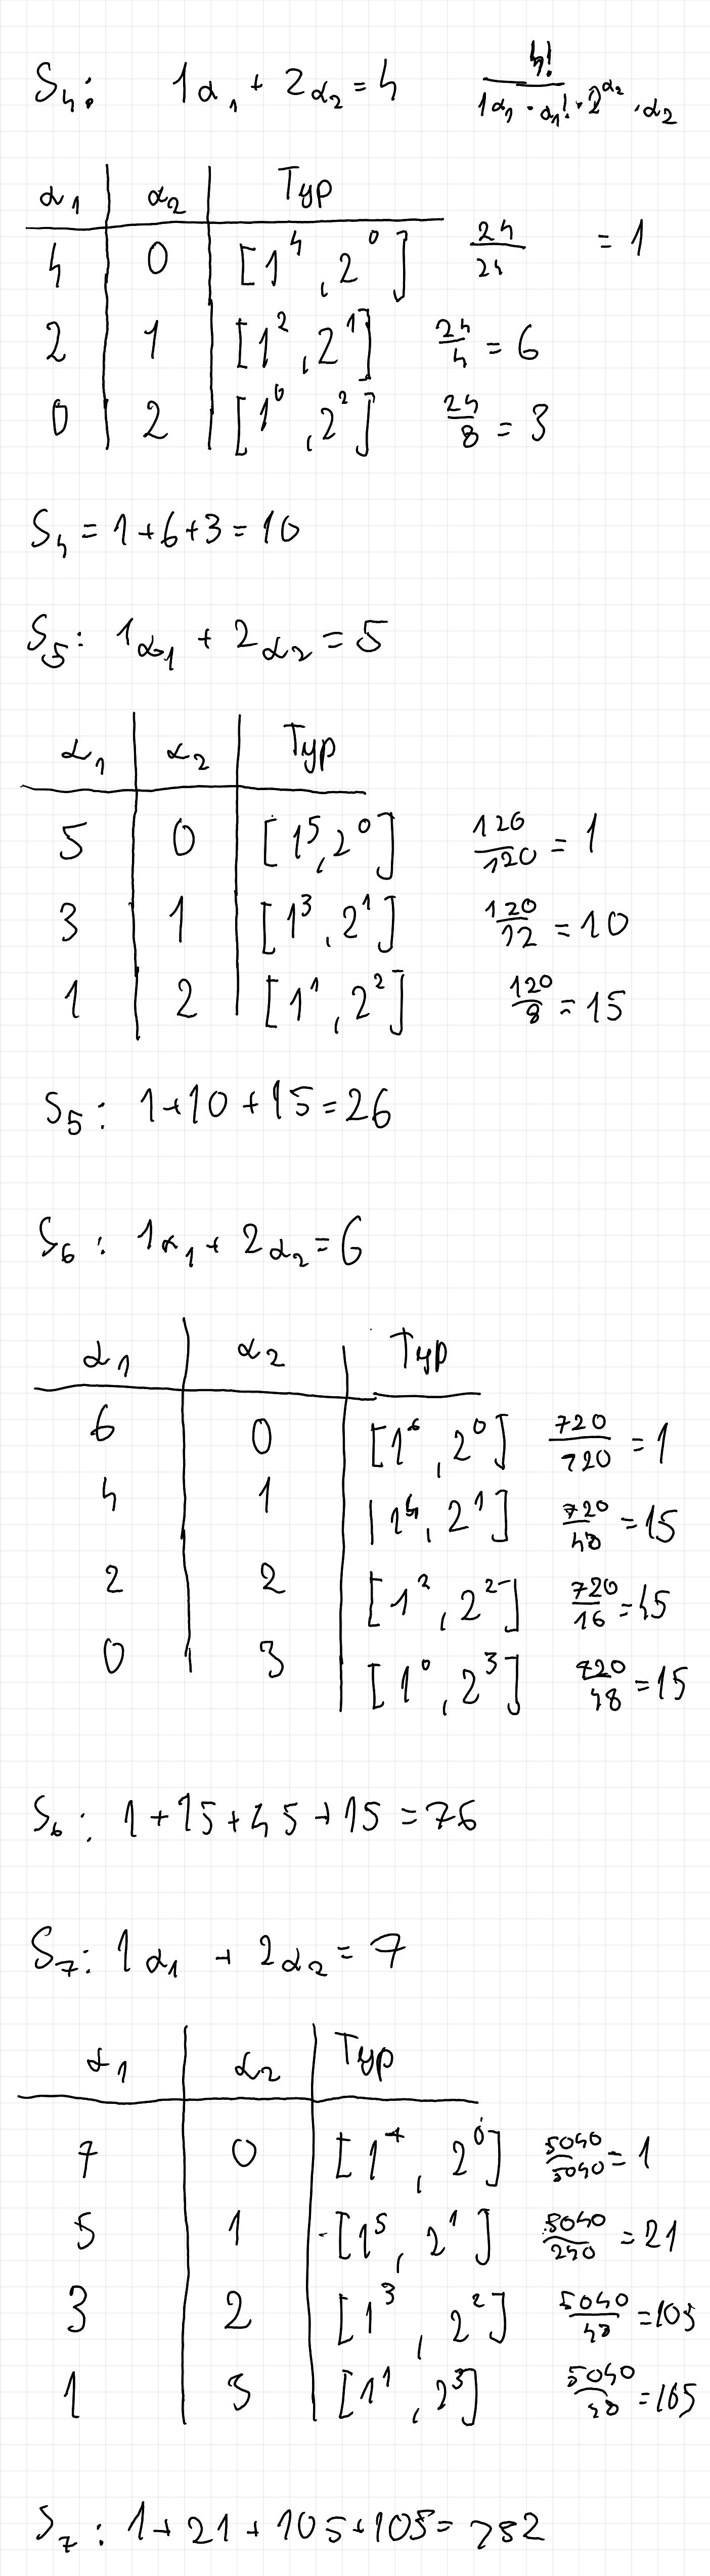
\includegraphics[width=0.45\textwidth]{zad 3b.png}
    \caption{Kombinatoryczne wyznaczanie liczby inwolucji dla $S_4, S_5, S_6, S_7$.}
    \label{fig:zad3b_reczne}
\end{figure}

\textbf{Opis do Rysunku \ref{fig:zad3b_reczne}:}
Dla wymiarów od $n=4$ do $n=7$ wypisano możliwe struktury cyklowe inwolucji. Zastosowano wzór Cauchy'ego: $\frac{n!}{1^{\alpha_1}\alpha_1! 2^{\alpha_2}\alpha_2!}$. Sumując wyniki dla dopuszczalnych typów cyklowych otrzymano łączną liczbę inwolucji: 10 (dla $S_4$), 26 (dla $S_5$), 76 (dla $S_6$) oraz 232 (dla $S_7$).

\begin{figure}[H]
    \centering
    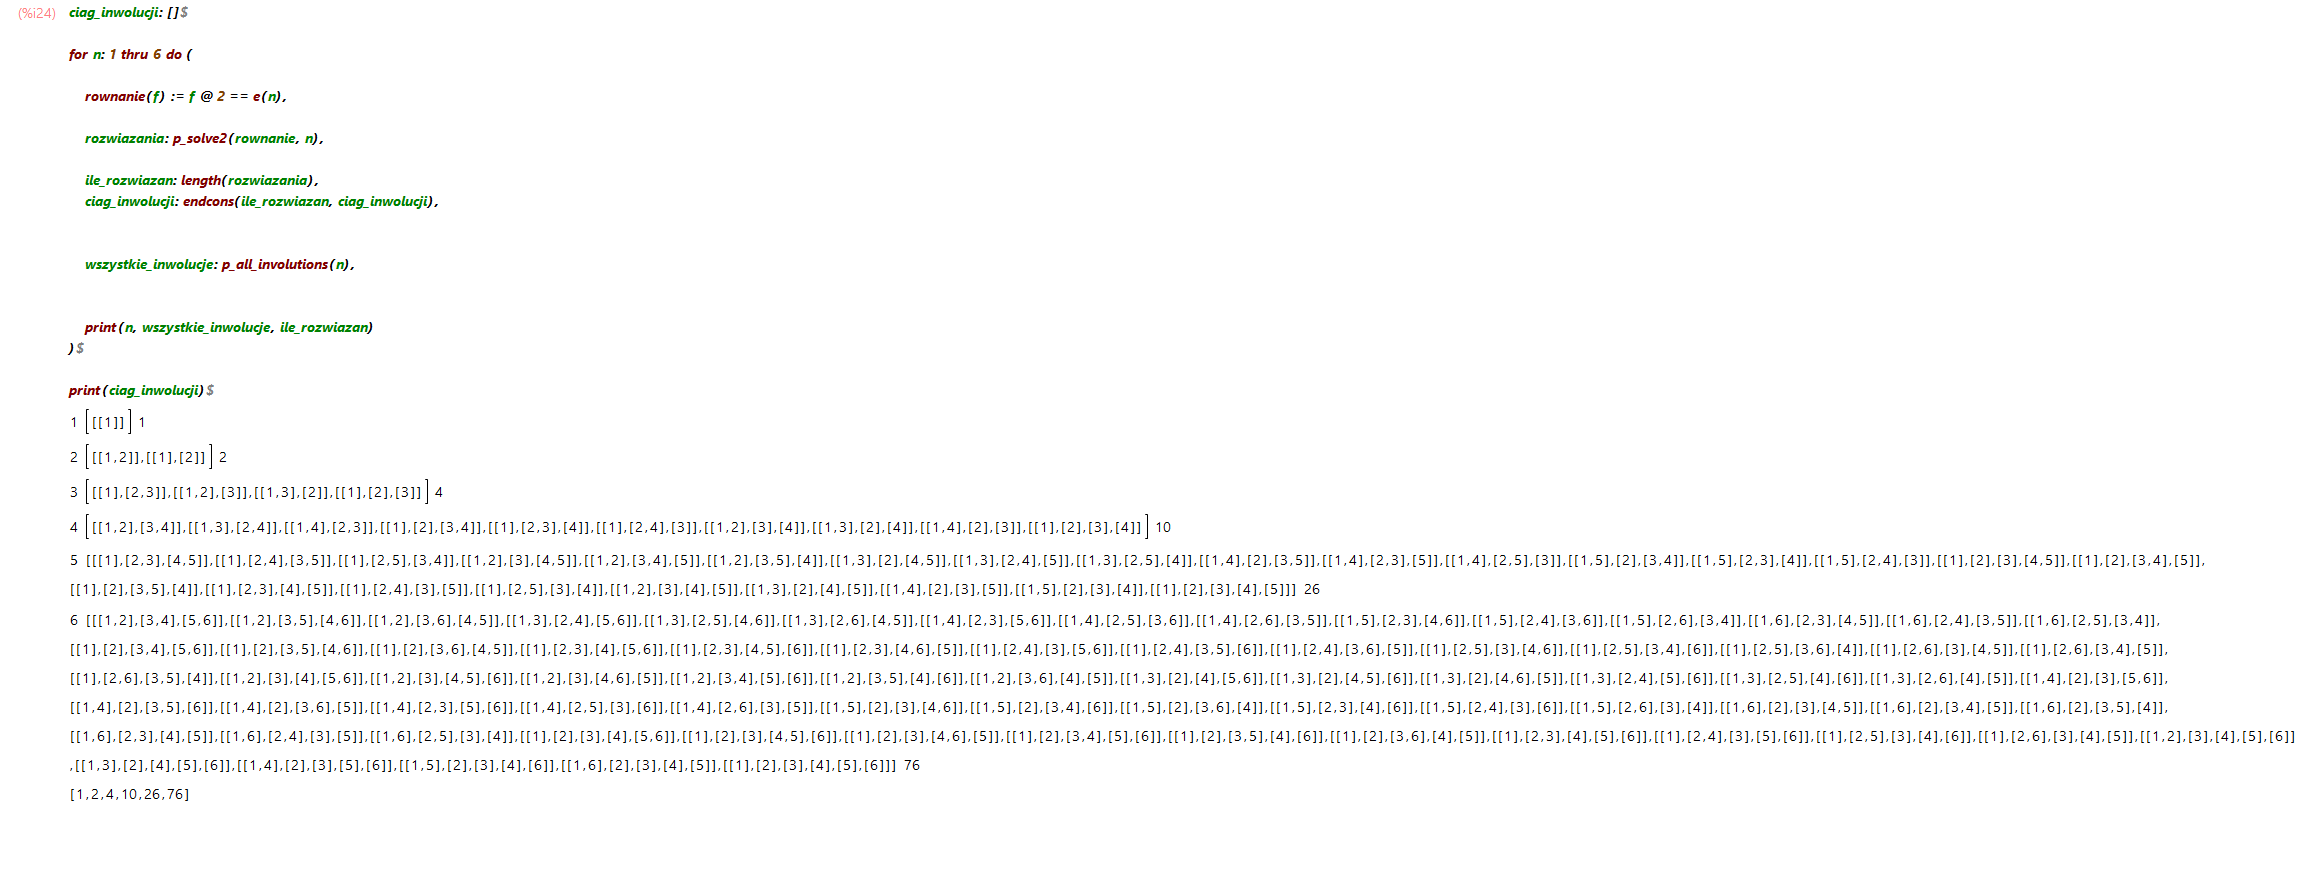
\includegraphics[width=0.95\textwidth]{zad 3b maxima.png}
    \caption{Skrypt generujący liczbę inwolucji w programie Maxima.}
    \label{fig:zad3b_maxima}
\end{figure}

\textbf{Opis do Rysunku \ref{fig:zad3b_maxima}:}
Działanie pętli generującej inwolucje w Maximie na podstawie weryfikacji warunku $f \circ f = e$. Wektor wyników pokrywa się z wyliczeniami analitycznymi.

\clearpage

\section{Zadanie 5: Wyznaczanie inwersji w permutacji}

\begin{figure}[H]
    \centering
    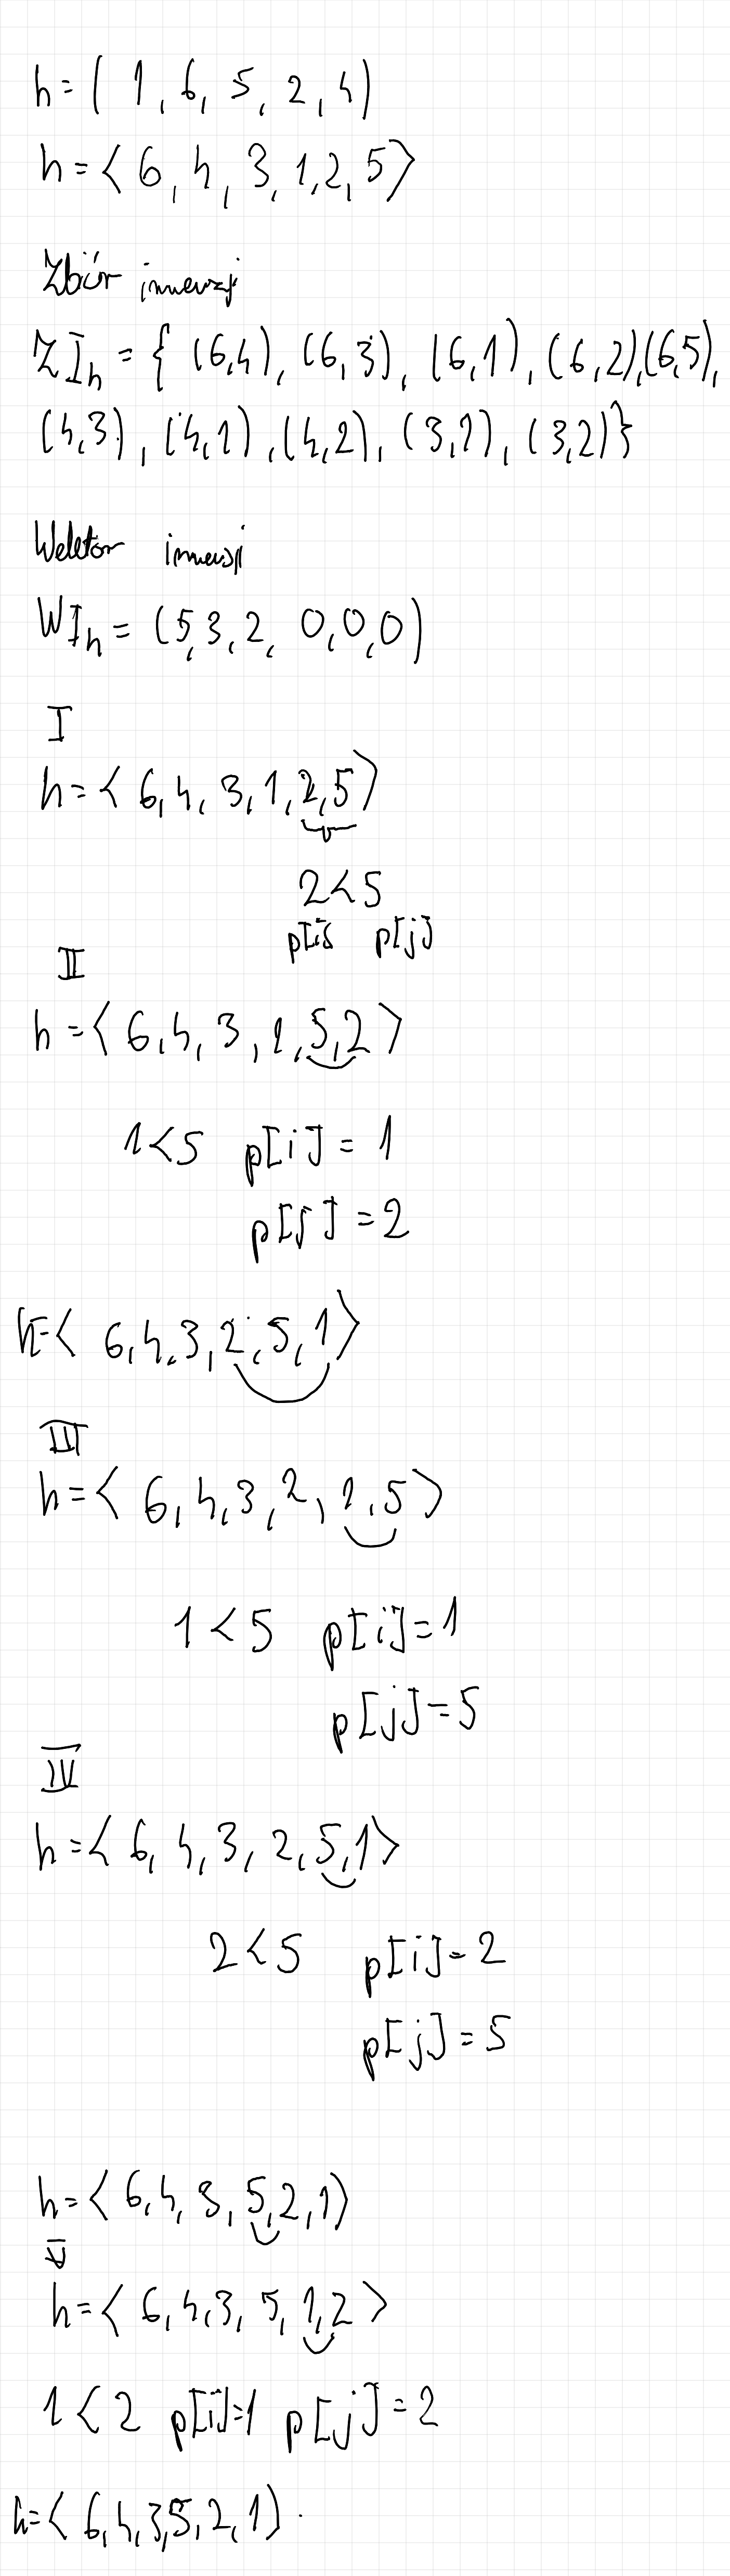
\includegraphics[width=0.4\textwidth]{zad5.png}
    \caption{Analiza inwersji permutacji $h$.}
    \label{fig:zad5_reczne}
\end{figure}

\textbf{Opis do Rysunku \ref{fig:zad5_reczne}:}
Dla $h = \langle 6, 4, 3, 1, 2, 5 \rangle$ wypisano zbiór inwersji (pary elementów, gdzie większy stoi przed mniejszym). Obliczono wektor inwersji $W_{I_h} = (5, 3, 2, 0, 0, 0)$.

\begin{figure}[H]
    \centering
    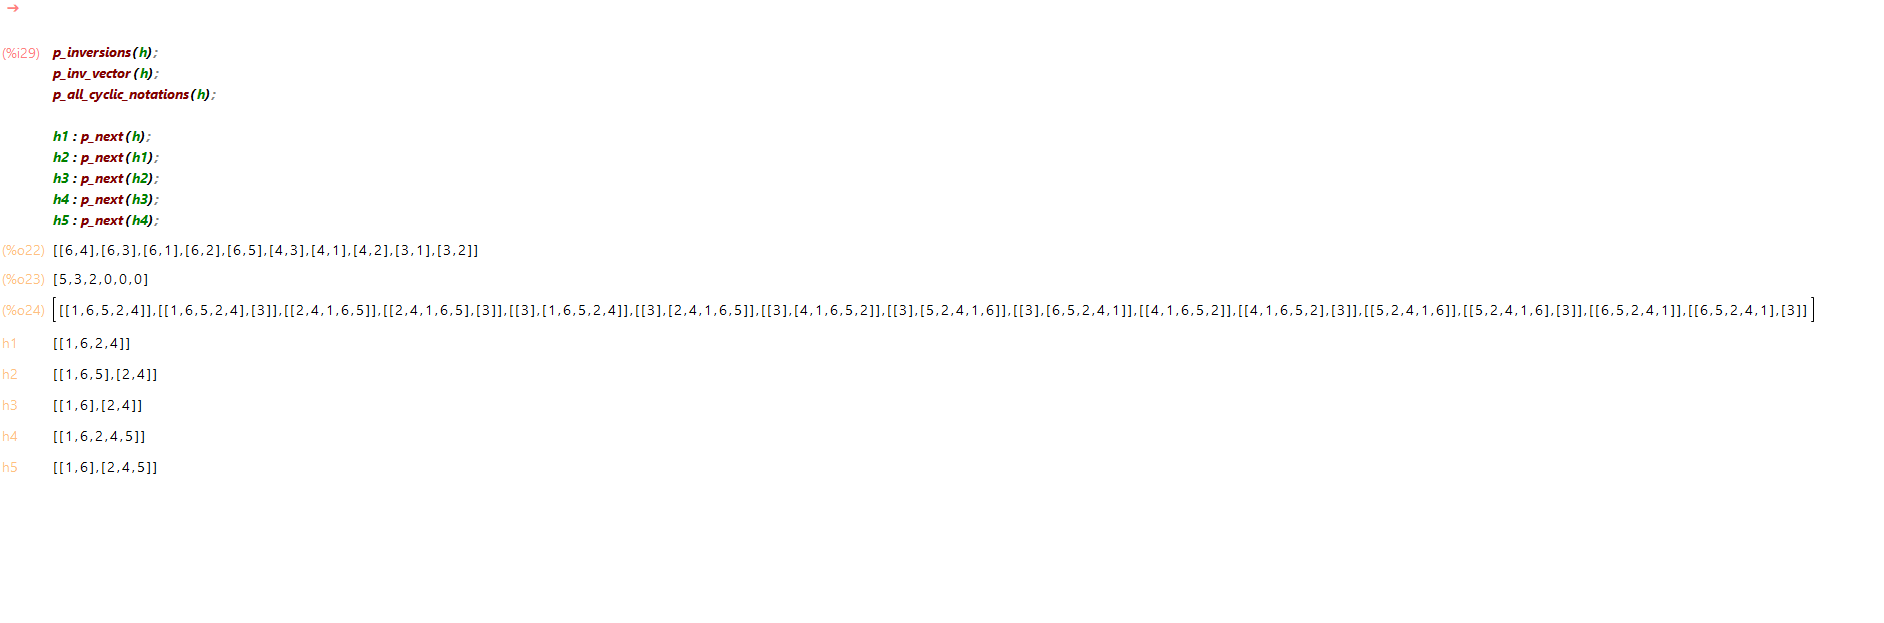
\includegraphics[width=0.9\textwidth]{zad 5 maxima.png}
    \caption{Wyznaczenie własności permutacji $h$ przez komputer.}
    \label{fig:zad5_maxima}
\end{figure}

\textbf{Opis do Rysunku \ref{fig:zad5_maxima}:}
Funkcje pakietu kombinatorycznego Maximy poprawnie wygenerowały wynik \texttt{[5, 3, 2, 0, 0, 0]}.

\clearpage

\section{Zadanie 10: Obliczanie liczby permutacji zadanego typu}

\begin{figure}[H]
    \centering
    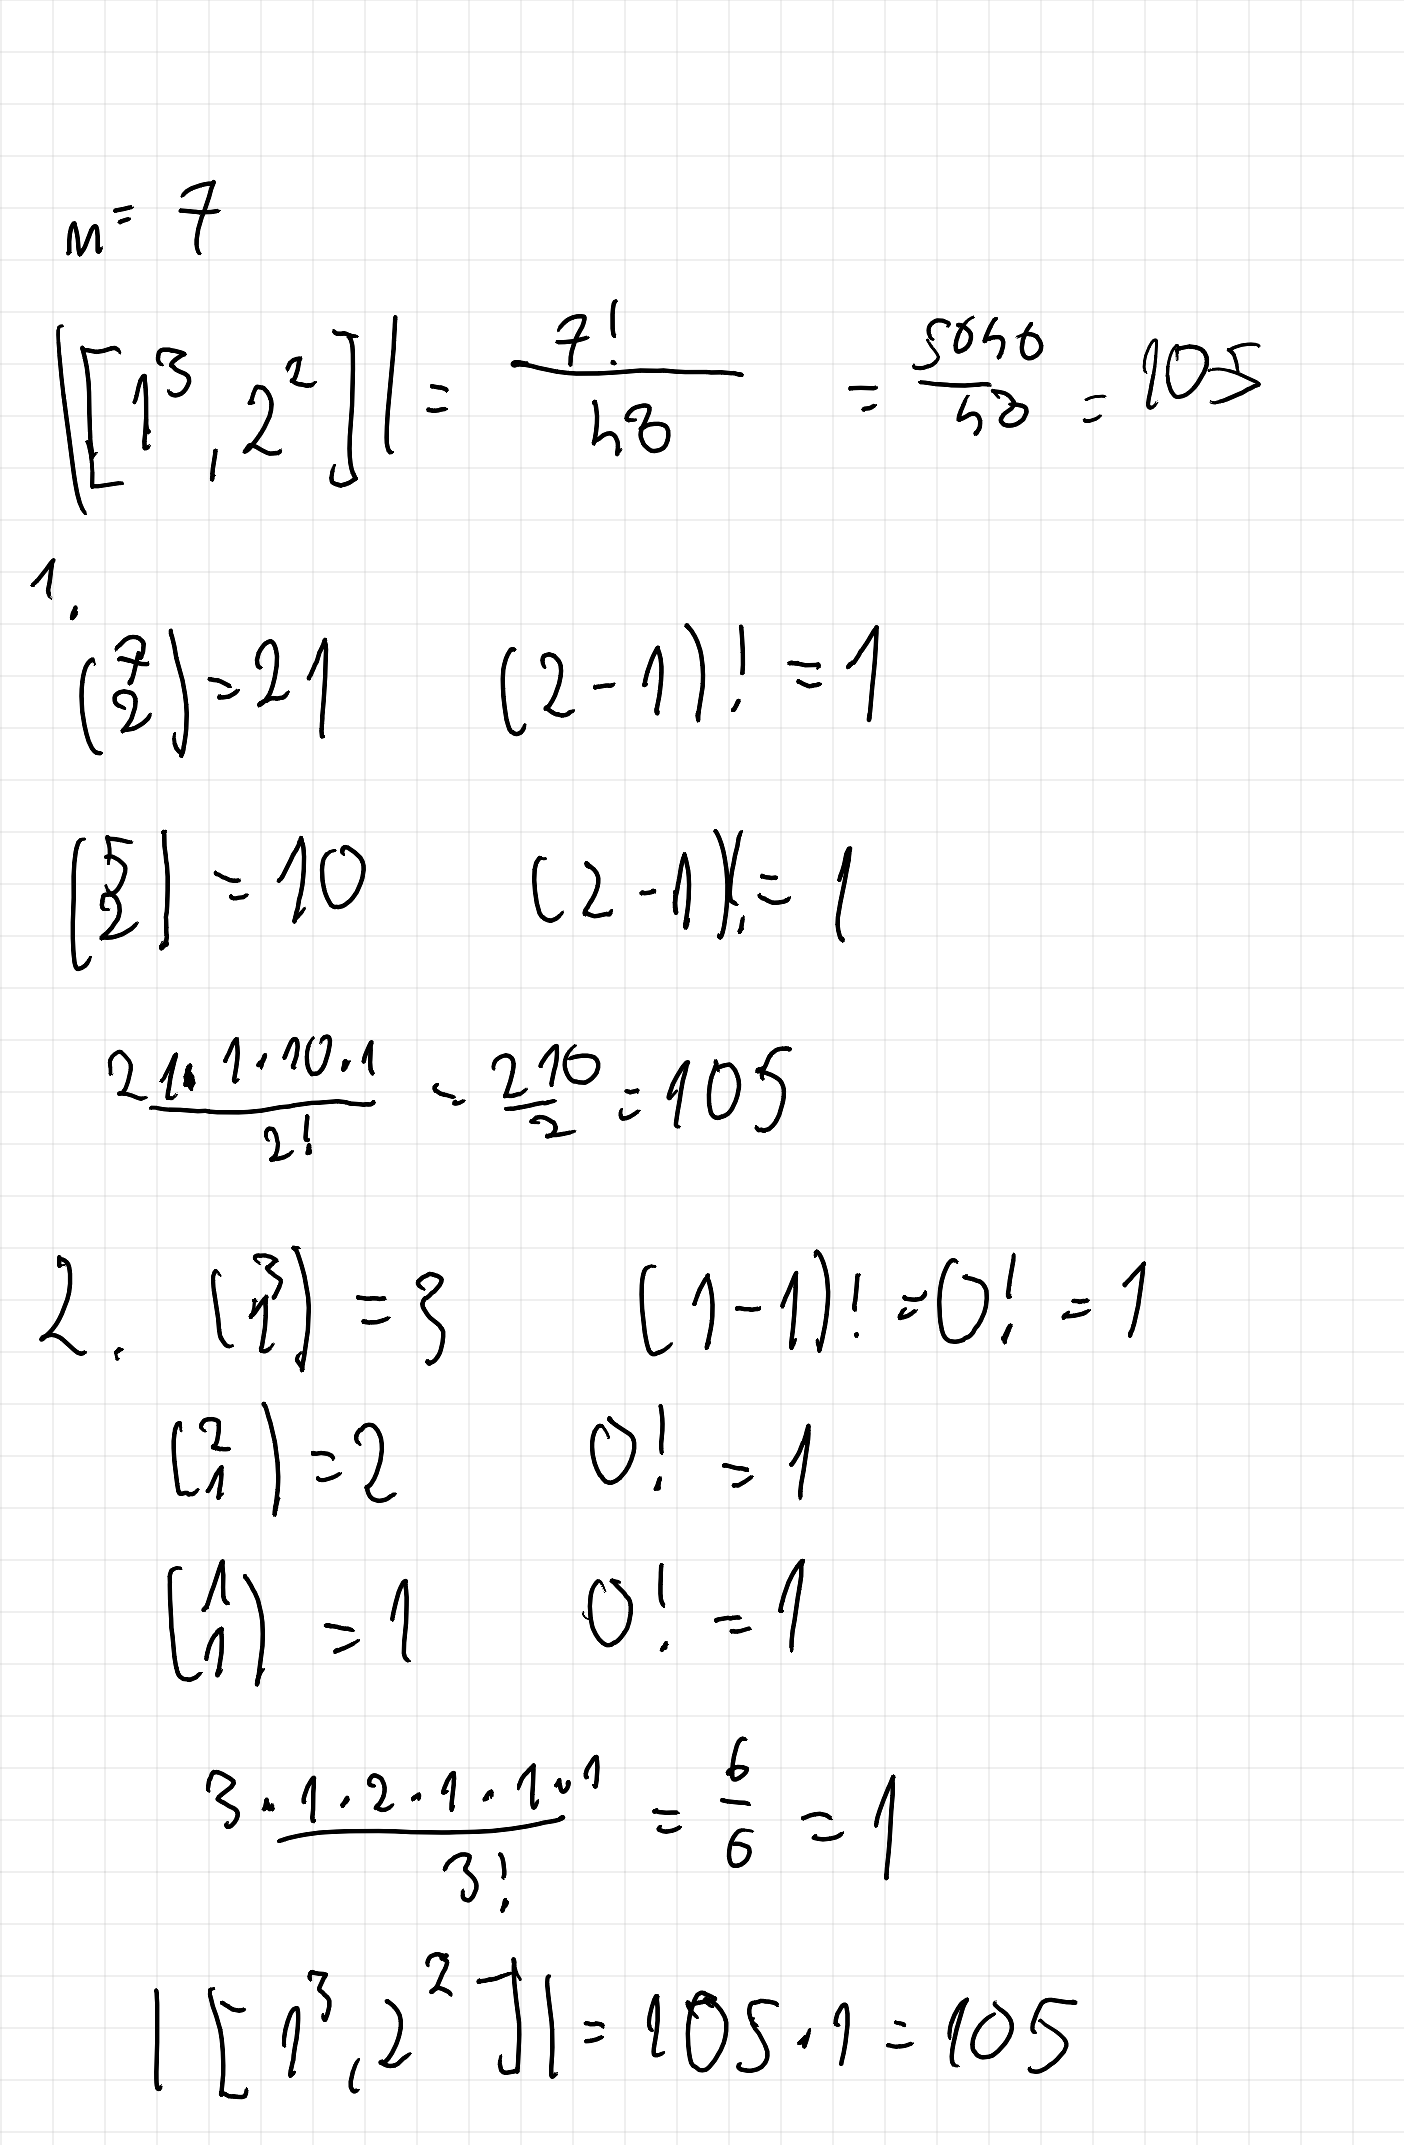
\includegraphics[width=0.55\textwidth]{zad 10.png}
    \caption{Obliczenie liczebności typu cyklowego w grupie $S_7$.}
    \label{fig:zad10_reczne}
\end{figure}

\textbf{Opis do Rysunku \ref{fig:zad10_reczne}:}
Obliczono liczbę permutacji o strukturze cyklowej $[1^3, 2^2]$ w grupie $S_7$, uzyskując wynik 105. Potwierdzono to na dwa sposoby: wzorem Cauchy'ego oraz metodą kombinatoryczną (z użyciem symbolu Newtona).

\begin{figure}[H]
    \centering
    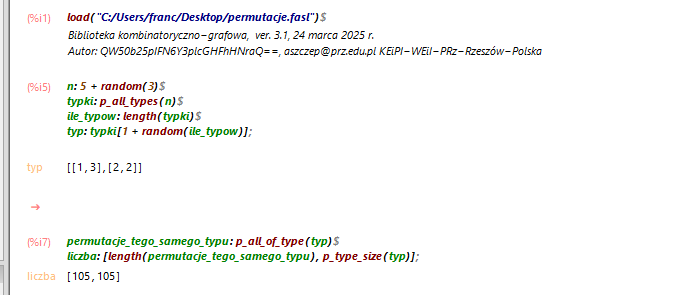
\includegraphics[width=0.8\textwidth]{zad 10 maxima.png}
    \caption{Weryfikacja rozmiaru klasy sprzężoności w programie Maxima.}
    \label{fig:zad10_maxima}
\end{figure}

\textbf{Opis do Rysunku \ref{fig:zad10_maxima}:}
Skrypt w Maximie zliczył permutacje pasujące do schematu, ostatecznie zwracając wartość 105.

\section{Podsumowanie}
Wykonana dokumentacja potwierdza całkowitą zgodność analiz analitycznych, przeprowadzonych krok po kroku metodami z dziedziny algebry i kombinatoryki, z wynikami maszynowymi z systemu Maxima. Prawidłowy podział skomplikowanych obliczeń na mniejsze etapy ułatwił weryfikację i minimalizację błędów na poszczególnych szczeblach analizy.

\end{document}